%%%%%%%%%%%%%%%%%%%% author.tex %%%%%%%%%%%%%%%%%%%%%%%%%%%%%%%%%%%
%
% sample root file for your "contribution" to a contributed volume
%
% Use this file as a template for your own input.
%
%%%%%%%%%%%%%%%% Springer %%%%%%%%%%%%%%%%%%%%%%%%%%%%%%%%%%


% RECOMMENDED %%%%%%%%%%%%%%%%%%%%%%%%%%%%%%%%%%%%%%%%%%%%%%%%%%%
\documentclass[graybox]{svmult}

% choose options for [] as required from the list
% in the Reference Guide

\usepackage{type1cm}        % activate if the above 3 fonts are
                            % not available on your system
%
\usepackage{makeidx}         % allows index generation
\usepackage{graphicx}        % standard LaTeX graphics tool
                             % when including figure files
\usepackage{multicol}        % used for the two-column index
\usepackage[bottom]{footmisc}% places footnotes at page bottom


\usepackage{newtxtext}       % 
\usepackage{newtxmath}       % selects Times Roman as basic font

\usepackage{booktabs}       % Booktabs Table Style
	
\usepackage{graphicx}       % To frame graphic images
\usepackage[export]{adjustbox}

\usepackage[section]{placeins} % Forces an image to be displayed in it's section
%\usepackage{draftwatermark}


% see the list of further useful packages
% in the Reference Guide

\makeindex             % used for the subject index
                       % please use the style svind.ist with
                       % your makeindex program

%%%%%%%%%%%%%%%%%%%%%%%%%%%%%%%%%%%%%%%%%%%%%%%%%%%%%%%%%%%%%%%%%%%%%%%%%%%%%%%%%%%%%%%%%

\DeclareUnicodeCharacter{2212}{-}
\DeclareUnicodeCharacter{22C5}{-}

\begin{document}

%\SetWatermarkText{DRAFT}
%\SetWatermarkScale{1}


\title*{A new breeding crossover approach for evolutionary algorithms}
%


\titlerunning{Animal Life Cycle Algorithm (ALCA)}
% Use \titlerunning{Short Title} for an abbreviated version of
% your contribution title if the original one is too long
\author{J. C. Felix-Saul, Mario García-Valdez}
% Use \authorrunning{Short Title} for an abbreviated version of
% your contribution title if the original one is too long
\institute{J. C. Felix-Saul \at TecNM, Tijuana Institute of Technology, Tijuana, Mexico, \email{jose.felix201@tectijuana.edu.mx}
\and Mario García-Valdez \at TecNM, Tijuana Institute of Technology, Tijuana, Mexico, \email{mario@tectijuana.edu.mx}}
%
% Use the package "url.sty" to avoid
% problems with special characters
% used in your e-mail or web address
%
\maketitle

\abstract*{In a previous work, we introduced a population-based, bio-inspired algorithm. The proposed algorithm is inspired by the biological animal life cycle, consisting of the stages of birth, growth, reproduction, and death. Our algorithm was initially based on the canonical Genetic Algorithm (GA), where all the individuals have a genotype (chromosome). One difference to highlight in our algorithm is that both the crossing and the mutation are executed through independent processes that randomly affect the population. This paper focuses on breeding, whereas in earlier versions of the algorithm, we used the traditional GA one-point crossover. In this paper, we propose a different alternative to the classical approach, where part of the genetic information is directly copied to each of the offspring in the crossover operator, where this type of crossover may not perform well in continuous optimization problems. In this proposal, we use the parent's genetic information for each gene, using those values as lower and upper bounds of a range, where a random value within that range determines the new value for that gene index of the offspring. This is similar to what is used by algorithms such as Differential Evolution, where we consider our proposal as a variation of existing proposals. We expect this new operator to allow the offspring to continue exploring new search spaces with the birth of individuals. In this paper, we use the benchmark functions introduced in the Competition on Evolutionary Computation for the 2017 edition (CEC2017) to compare the traditional one-point crossover and our proposed strategy. Experimental results indicate that our proposed operator may be a good alternative for the canonical crossover.}



\abstract{In a previous work, we introduced a population-based, bio-inspired algorithm. The proposed algorithm is inspired by the biological animal life cycle, consisting of the stages of birth, growth, reproduction, and death. Our algorithm was initially based on the canonical Genetic Algorithm (GA), where all the individuals have a genotype (chromosome). One difference to highlight in our algorithm is that both the crossing and the mutation are executed through independent processes that randomly affect the population. This paper focuses on breeding, whereas in earlier versions of the algorithm, we used the traditional GA one-point crossover. In this paper, we propose a different alternative to the classical approach, where part of the genetic information is directly copied to each of the offspring in the crossover operator, where this type of crossover may not perform well in continuous optimization problems. In this proposal, we use the parent's genetic information for each gene, using those values as lower and upper bounds of a range, where a random value within that range determines the new value for that gene index of the offspring. This is similar to what is used by algorithms such as Differential Evolution, where we consider our proposal as a variation of existing proposals. We expect this new operator to allow the offspring to continue exploring new search spaces with the birth of individuals. In this paper, we use the benchmark functions introduced in the Competition on Evolutionary Computation for the 2017 edition (CEC2017) to compare the traditional one-point crossover and our proposed strategy. Experimental results indicate that our proposed operator may be a good alternative for the canonical crossover.}

%\keywords{Distributed Bioinspired Algorithms \and Genetic Algorithms \and Cloud Computing.}

\newpage
\section{Introduction}
    \label{sec:1}

    Biologically inspired algorithms are a very effective technique to solve complex optimization problems\cite{castillo2019comparative,valdez2021swarm,acherjee2020ultrasonic}. Traditionally, nature-inspired algorithms are developed with a sequential perspective\cite{porto2018evolutionary,back1996evolutionary},  meaning that all tasks execute one step at a time, where all processes must wait for the previous to finish before continuing (synchronous perspective). Some architectures address this issue by working on the cloud\cite{valdez2021container,garcia2015evospace,merelo2016nodio} and finding solutions on distributed technologies. 
    
    In previous work, we introduced a population-based, bio-inspired algorithm\cite{Felix-Saul2022,Felix-Saul2023}. The proposed algorithm is inspired by the biological animal life cycle, consisting of the stages\cite{read1968system} of birth, growth, reproduction, and death. Our algorithm was initially based on the canonical Genetic Algorithm (GA)\cite{holland1992genetic,holland1984genetic}, where all the individuals have a genotype (chromosome). Our algorithm’s goal is to mimic the animal life cycle, where at any given moment, new individuals are born to be part of the population and participate in the collective evolution. As time passes, they grow older and mature, suffering changes throughout their lives that we chose to represent as mutations. 

    In our analysis, we thought of death’s work to maintain balance in the population by enforcing the survival of the fittest. As in life, death can happen to everyone: from a newborn to the elderly, where fitness will determine the individual’s longevity. This algorithm was inspired by the traditional Genetic Algorithm \cite{holland1992genetic,holland1984genetic}, meaning that all individuals have a genotype (chromosome) that is a list of values. We calculate the individual’s fitness with the evaluation function and do crossover and mutation to the population. 
    
    What makes our strategy different is that we don’t use the concept of evolutionary generations. We manage our set of solutions as a whole that continuously evolve over time. Allowing individuals of different ages to breed and generate offspring, as it happens in nature. One difference to highlight in our algorithm is that both the crossover (reproduction) and mutation (growth) are executed through independent processes that randomly affect the population. We display the general model concept for the Animal Life Cycle Algorithm (ALCA) in Figure~\ref{fig.algorithm_model}. 

    In this research, we propose a new alternative for reproduction, a new breeding crossover approach for evolutionary algorithms using the classic one-point crossover as a reference to our proposal. We performed comparison experiments using the mathematical benchmark functions introduced in the Competition on Evolutionary Computation for the 2017 edition (CEC-2017) for evaluation. We finalize with a statistical Z-Test with a 95 percent confidence level to determine the best alternative.

    We organized this paper in the following structure. First, we illustrate our alternative crossover proposal, from the inspiration to a detailed example. We compare the canonical one-point crossover with our proposed solution in section~\ref{section.proposal}, followed by our experiment configuration and results in section~\ref{section.experiments}, where we analyze and describe some of our research findings in section~\ref{section.discussion}. We finalize by presenting some inferences based on the results of our experiments in section~\ref{section.conclusions}.

    \begin{figure}[!ht]
        \centering
        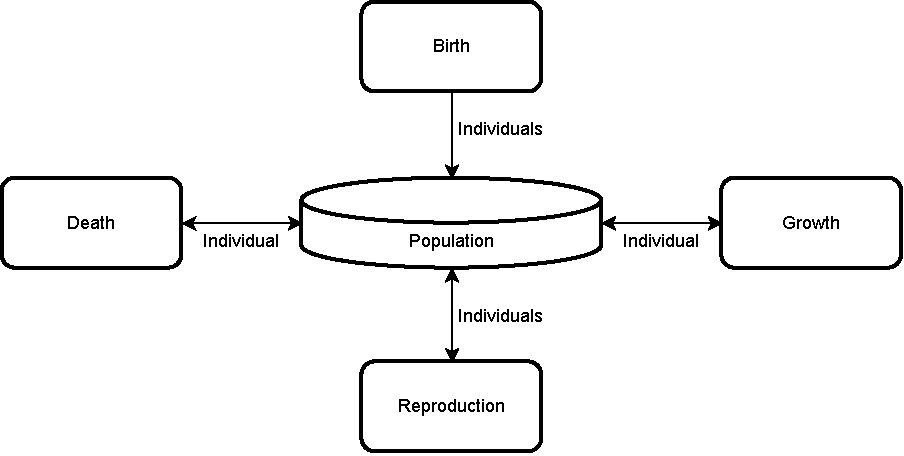
\includegraphics[width=0.90\linewidth]{img/fig_algorithm_model.pdf}
        \caption{Animal Life Cycle Algorithm model.} \label{fig.algorithm_model}
        \end{figure}


\section{Proposal}
    \label{section.proposal}

    Let's imagine that colors black and white fell in love and had beautiful children. If we had to guess what color their offspring would be, it could only be predictable its children's color would be inside the domain shown in Figure~\ref{fig.grayscale_continuous}.

    \begin{figure}[!ht]
        \centering
        
\includegraphics[width=0.70\linewidth]{img/fig_grayscale_continuous.pdf}
        \caption{Black and white offspring predictable color domain.} \label{fig.grayscale_continuous}
        \end{figure}

    If we replace colors black and white with values 0 and 1 respectively, how many values can we find in between? We could replace attributes, switching from color to height, strength, agility, or any other feature we might need to focus on. The parents' attribute values will determine how their offspring's attributes are defined. This paper focuses on breeding (or reproduction), whereas in earlier versions of the algorithm, we used the traditional (GA) one-point crossover. 

    \subsection{Crossover Proposal}

    In this paper, we propose a different alternative to the classical approach, where part of the genetic information is directly copied to each of the offspring in the crossover operator, where this type of crossover may not perform well in continuous optimization problems. We provide an example of the One Point Crossover in Figure~\ref{fig.onepoint_crossover}.

    \begin{figure}[!ht]
        \centering
        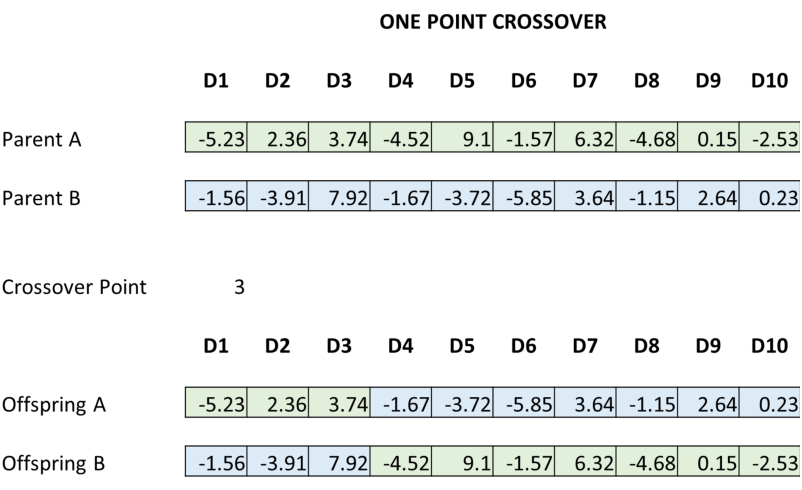
\includegraphics[width=0.70\linewidth]{img/fig_onepoint_crossover.pdf}
        \caption{Classical approach example for the One Point Crossover, with crossover point 3.} \label{fig.onepoint_crossover}
        \end{figure}

    In this proposal, we use the parent's genetic information for each gene, using those values as lower and upper bounds of a range, where a random value within that range determines the new value for that gene index of the offspring. Our proposal example for the Continuous Range Crossover is displayed in Figure~\ref{fig.contrange_crossover}, where it should be noted that we construct a template that will be used for all the offspring generated by each couple.

    \begin{figure}[!ht]
        \centering
        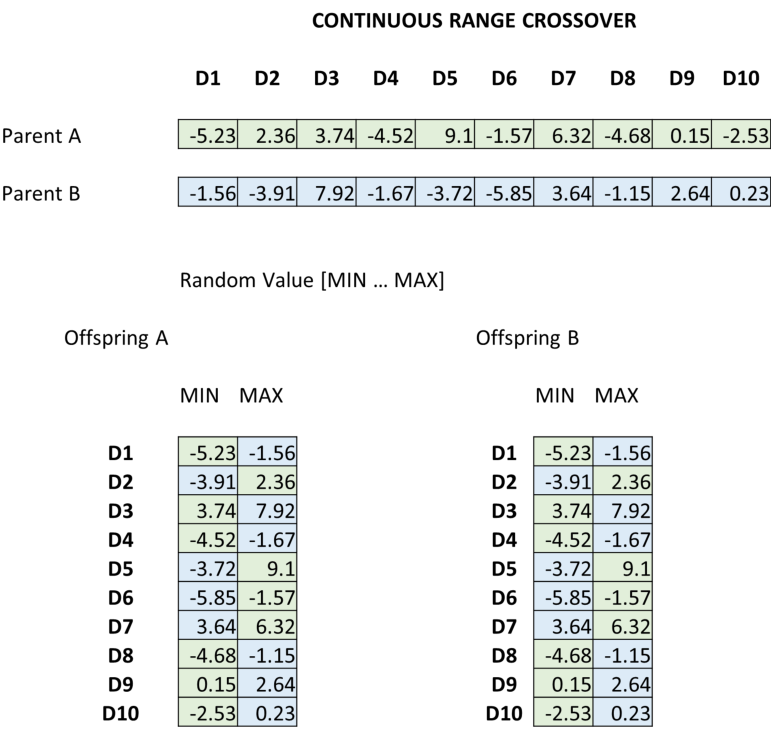
\includegraphics[width=0.70\linewidth]{img/fig_contrange_crossover.pdf}
        \caption{Our proposal example for the Continuous Range Crossover mating the same couple of individuals.} \label{fig.contrange_crossover}
        \end{figure}        
    
    \FloatBarrier


\section{Experiments}
    \label{section.experiments}

    To validate our proposal, we performed experiments using the mathematical benchmark functions introduced in the Competition on Evolutionary Computation for the 2017 edition (CEC-2017) for evaluation to compare the traditional one-point crossover and our proposed strategy. We finalize with a statistical Z-Test with a ninety-five percent confidence level to determine the best alternative. Table~\ref{tab.benchmark_functions} lists the thirty mathematical benchmark functions used for evaluation, to obtain the comparison results shown in our research.

    % Please add the following required packages to your document preamble:
    % \usepackage{booktabs}
    % \usepackage[table,xcdraw]{xcolor}
    % If you use beamer only pass "xcolor=table" option, i.e. \documentclass[xcolor=table]{beamer}
    \begin{table}[]
    \scriptsize
    \centering
    \caption{Mathematical benchmark functions introduced in the Competition on Evolutionary Computation for the 2017 edition (CEC-2017).}\label{tab.benchmark_functions}    
    \begin{tabular}{@{}cllcl@{}}
    \toprule
    \multicolumn{5}{c}{\textbf{CEC-2017 Mathematical Benchmark Functions}} \\ \midrule
    \textbf{Fx} & \textbf{Function Name} &  & \textbf{Fx} & \textbf{Function Name} \\
    F1 & Shifted and Rotated   Bent Cigar Function &  & F16 & Hybrid function 6 \\
    F2 & Shifted and Rotated   Sum of Different Power Function &  & F17 & Hybrid function 7 \\
    F3 & Shifted and Rotated   Zakharov Function &  & F18 & Hybrid function 8 \\
    F4 & Shifted and Rotated   Rosenbrock's Function &  & F19 & Hybrid function 9 \\
    F5 & Shifted and Rotated   Rastrigin's Function &  & F20 & Hybrid function 10 \\
    F6 & Shifted and Rotated   Schaffer F7 Function &  & F21 & Composition function   1 \\
    F7 & Shifted and Rotated   Lunacek Bi-Rastrigin's Function &  & F22 & Composition function   2 \\
    F8 & Shifted and Rotated   Non-Continuous Rastrigin's Function &  & F23 & Composition function   3 \\
    F9 & Shifted and Rotated   Levy Function &  & F24 & Composition function   4 \\
    F10 & Shifted and Rotated   Schwefel's Function &  & F25 & Composition function   5 \\
    F11 & Hybrid function 1 &  & F26 & Composition function   6 \\
    F12 & Hybrid function 2 &  & F27 & Composition function   7 \\
    F13 & Hybrid function 3 &  & F28 & Composition function   8 \\
    F14 & Hybrid function 4 &  & F29 & Composition function   9 \\
    F15 & Hybrid function 5 &  & F30 & Composition function   10 \\ \bottomrule
    \end{tabular}
    \end{table}


    \subsection{Experimental Configuration}

    We used the Animal Life Cycle Algorithm (ALCA) for our experiments, switching between the breeding strategies (One Point and Continuous Range Crossover) with the same general setup. In Table~\ref{tab.general_configuration}, we can find the General Configuration used to run the experiments for our research, where all values from this configuration remained constant during all phases of the experiment runs.

    For each of the thirty mathematical benchmark functions from the CEC-2017, we evaluated the ten and thirty dimensions, where we performed fifty-one runs per dimension. To find and determine the best alternative finalized with a statistical Z-Test with a ninety-five percent confidence level.

    % Please add the following required packages to your document preamble:
    % \usepackage{booktabs}
    % \usepackage[table,xcdraw]{xcolor}
    % If you use beamer only pass "xcolor=table" option, i.e. \documentclass[xcolor=table]{beamer}
    \begin{table}[]
    \scriptsize
    \centering
    \caption{Animal Life Cycle Algorithm (ALCA) General Configuration.}\label{tab.general_configuration}    
    \begin{tabular}{@{}ll@{}}
    \toprule
    \multicolumn{2}{l}{\textbf{ALCA   General Configuration}} \\ \midrule
    \textbf{Function name} & \textbf{ALL} \\
    Population & 500 \\
    Evaluations & 10,000 * Dim \\
    Crossover rate & 100 \\
    Mutation rate & 7 \\
    Max age & 5 \\
    Tournament rep. & 100 \\
    Sample size & 20 \\
    Base approval & 80 \\
    Goal approval & 200 \\ \bottomrule
    \end{tabular}
    \end{table}

    \FloatBarrier


    \subsection{Experimental Results}

    We describe how to interpret the results presented in our Box and Whisker charts for each mathematical function. We display the ten and thirty-dimension charts on the left and right sides. We can find the results accumulated in 51 runs, in green color the One Point crossover, and in blue color the Continuous Range crossover. The closer the error results get to the zero value, the better.

    
    STOP HERE --- A new beginning (this is an upload test).    


        For each experiment, we ran 30 independent executions per algorithm and
        dimensions specified. We recorded the following results: best-found error average,
        standard deviation, total number of evaluations, and total elapsed time (in
        seconds). The labels used on the results of our summarized experiments tables
        are the following:

        \begin{itemize}
            \item   Error:       is the best-found error average.
            \item   St-Dev:      is the standard deviation calculated from the error. 
            \item   Evals.:      is the total number of evaluations the algorithm executed.
            \item   Time:        is the total elapsed or wall clock time, in seconds. 
        \end{itemize}

        The alternatives to restart this new population are the creation of a new set
        of candidate solutions based on either: 1. Crossing the Champion with the Elite;
        2. The mutation with uniform modification from the Elite; 3. The
        projection of the Elite towards the Champion; 4. Based on random use of the
        previous alternatives. We compared three strategies by grouping the previous
        alternatives in the following:

        \begin{itemize}
            \item   Xover Mutation:      Crossing the Champion with the Elite, and the mutation with uniform modification from the Elite.
            \item   Elite Projection:    The projection of the Elite towards the Champion. 
            \item   All Random:          Based on random use of the previous alternatives.
        \end{itemize}

        \subsubsection{Ackley Benchmark Function Experiment}

            The goal of the first experiment was to confirm that this paper’s
            proposed strategy obtained improved results over our basic
            technique, which created a new population with a random generation
            of a new set of candidate solutions. We chose Ackley as the first
            Classic Benchmark Function for Optimization to test our algorithm
            behavior, where Figure~\ref{fig.fun_ackley} shows its corresponding
            Box and Whisker chart, and we summarized the results in
            Tables~\ref{tab.fun_ackley5} and~\ref{tab.fun_ackley10} (for five 
            and ten dimensions, respectively).
            
            \begin{figure}
                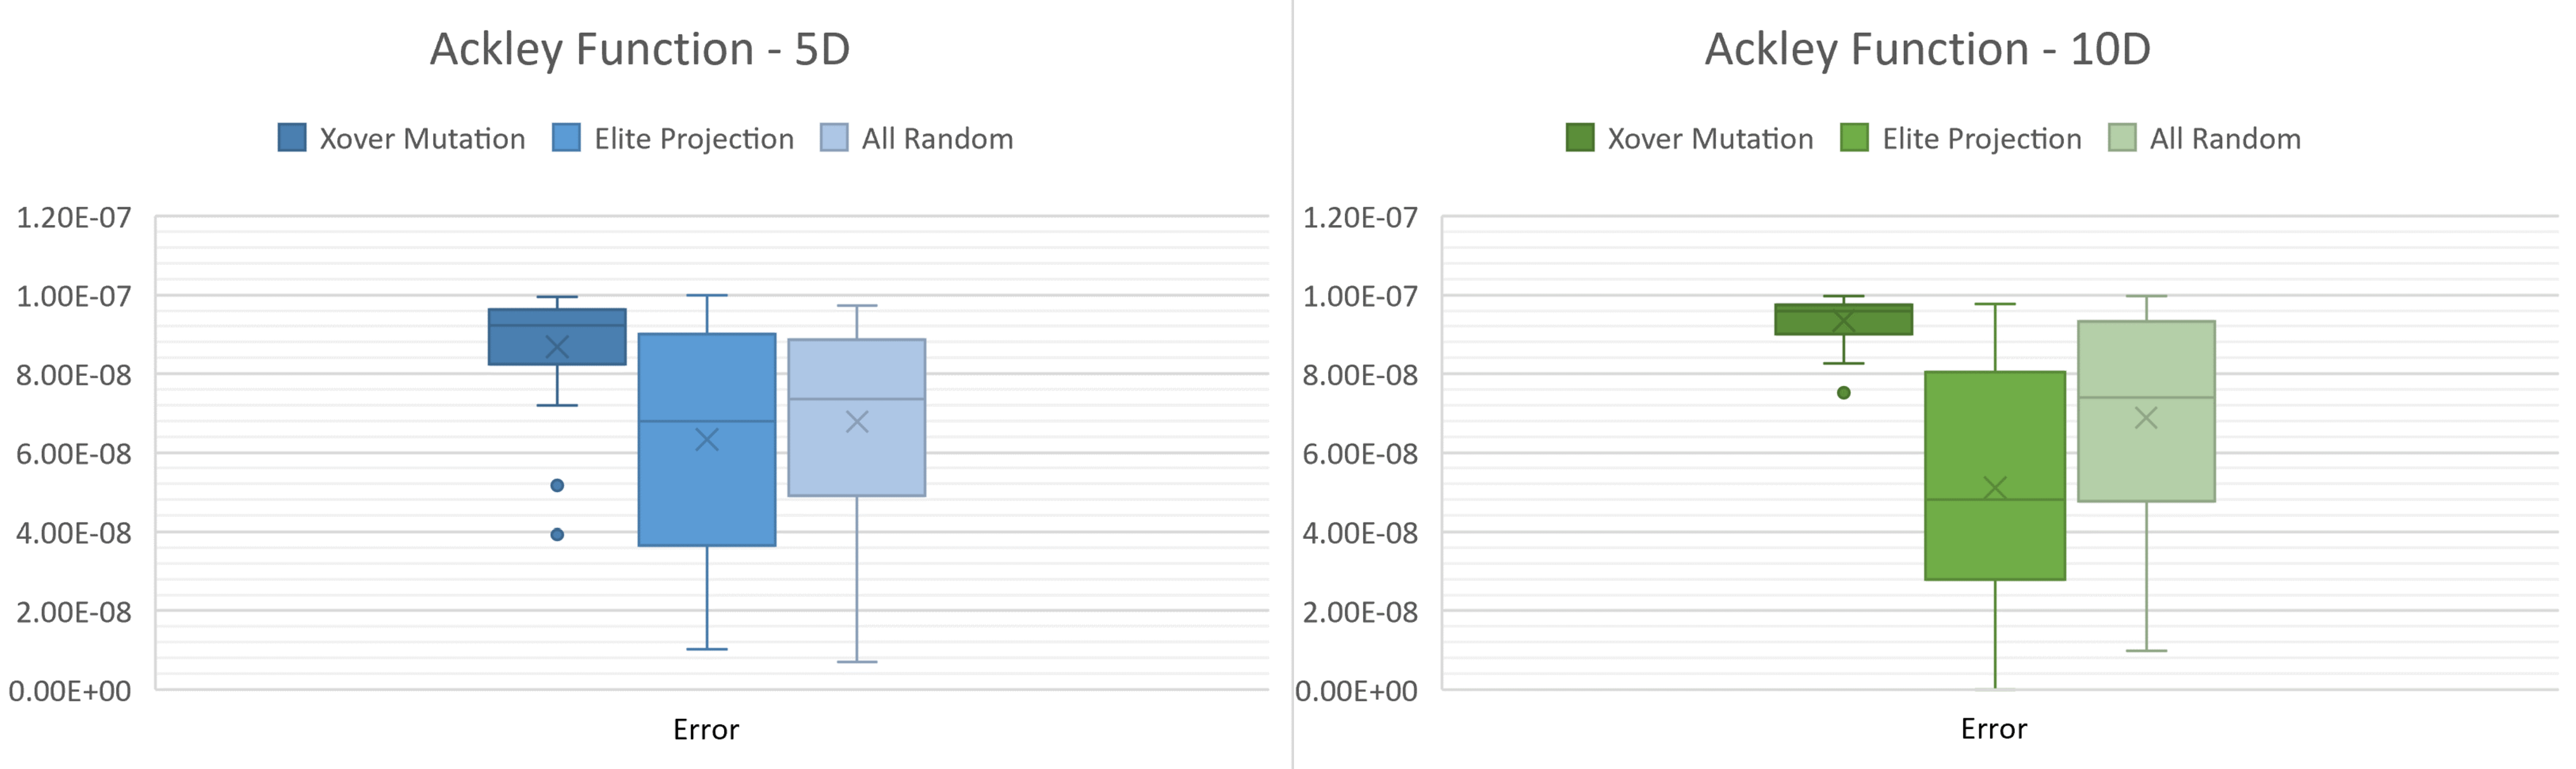
\includegraphics[width=0.99\linewidth, frame]{img/fig_fun_ackley.pdf}
                \caption{Box and whisker chart for the Ackley Benchmark Function, 5 vs 10 Dimensions.} \label{fig.fun_ackley}
                \end{figure}

            \begin{table}[]
                \scriptsize
                \centering
                \caption{Ackley Benchmark Function summarized experiments table for 5 Dimensions.}\label{tab.fun_ackley5}
                \begin{tabular}{@{}lllll@{}}
                \toprule
                \multicolumn{5}{l}{\textbf{Ackley Function - 5 Dimensions}} \\ \midrule
                & \textbf{Error} & \textbf{St-Dev} & \textbf{Evals.} & \textbf{Time} \\
                \textbf{Xover Mutation} & 8.69E-08 & 1.36E-08 & 46,331 & 49.9 \\
                \textbf{Elite Projection} & 6.33E-08 & 2.70E-08 & 13,811 & 18.1 \\
                \textbf{All Random} & 6.78E-08 & 2.55E-08 & 30,236 & 32.8 \\ \bottomrule
                \end{tabular}
                \end{table}

            \begin{table}[]
                \scriptsize
                \centering
                \caption{Ackley Benchmark Function summarized experiments table for 10 Dimensions.}\label{tab.fun_ackley10}
                \begin{tabular}{@{}lllll@{}}
                \toprule
                \multicolumn{5}{l}{\textbf{Ackley Function - 10 Dimensions}} \\ \midrule
                & \textbf{Error} & \textbf{St-Dev} & \textbf{Evals.} & \textbf{Time} \\
                \textbf{Xover Mutation} & 9.35E-08 & 5.93E-09 & 104,842 & 111.7 \\
                \textbf{Elite Projection} & 5.11E-08 & 3.13E-08 & 16,019 & 20.1 \\
                \textbf{All Random} & 6.89E-08 & 2.75E-08 & 43,631 & 46.3 \\ \bottomrule
                \end{tabular}
                \end{table}
            
            \FloatBarrier


        \subsubsection{Bohachevsky Benchmark Function Experiment}

            As our second experiment to further validate and prove our
            algorithm behavior, we chose Bohachevsky Classic Benchmark Function
            for Optimization. Figure~\ref{fig.fun_bohachevsky} shows its
            corresponding Box and Whisker chart, where we summarized the
            results in Tables~\ref{tab.fun_bohachevsky5} and~\ref{tab.fun_bohachevsky10} 
            (for five and ten dimensions, respectively). Due to the observation 
            and analysis of these results, we identify our proposed strategy 
            obtained solutions in the same order as the traditional Xover Mutation, 
            in a significantly reduced number of evaluations.

            \begin{figure}
                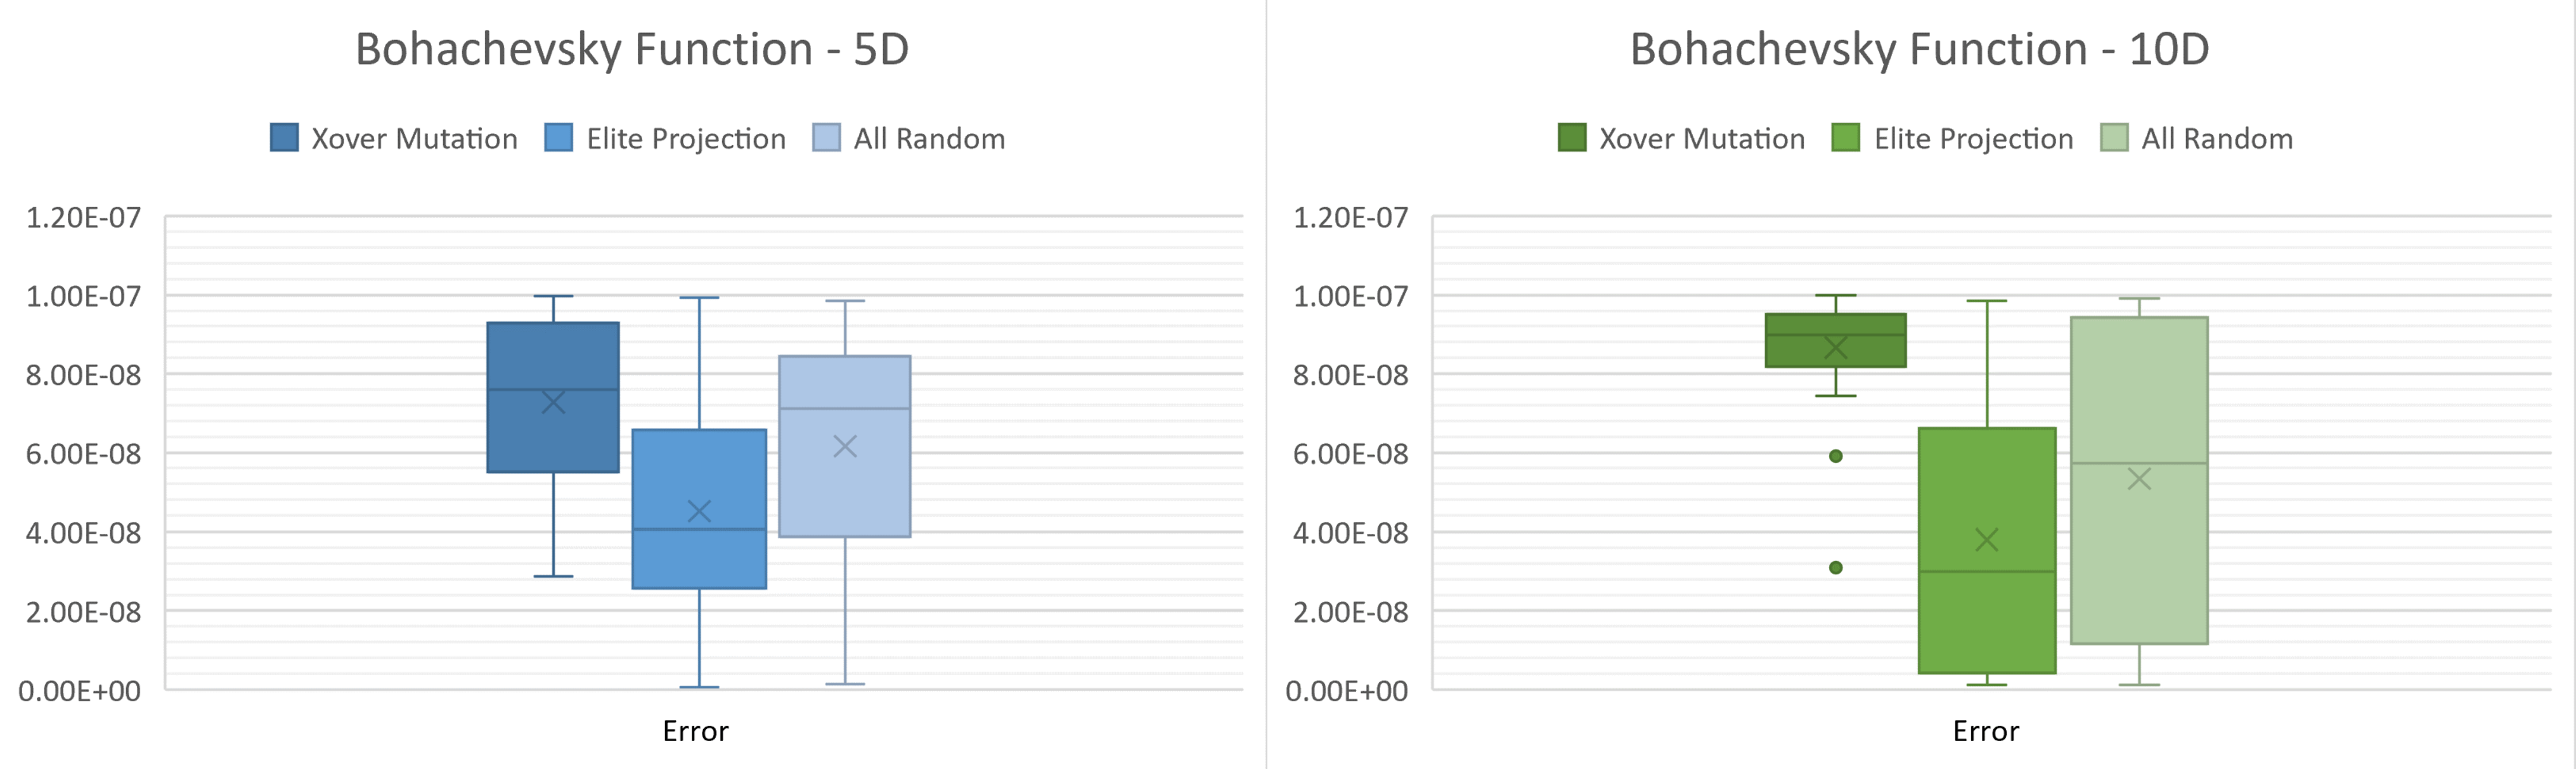
\includegraphics[width=0.99\linewidth, frame]{img/fig_fun_bohachevsky.pdf}
                \caption{Box and whisker chart for the Bohachevsky Benchmark Function, 5 vs 10 Dimensions.} \label{fig.fun_bohachevsky}
                \end{figure}

            \begin{table}[]
                \scriptsize
                \centering
                \caption{Bohachevsky Benchmark Function summarized experiments table for 5 Dimensions.}\label{tab.fun_bohachevsky5}
                \begin{tabular}{@{}lllll@{}}
                \toprule
                \multicolumn{5}{l}{\textbf{Bohachevsky Function - 5 Dimensions}} \\ \midrule
                & \textbf{Error} & \textbf{St-Dev} & \textbf{Evals.} & \textbf{Time} \\
                \textbf{Xover Mutation} & 7.28E-08 & 2.20E-08 & 15,010 & 24.2 \\
                \textbf{Elite Projection} & 4.51E-08 & 2.94E-08 & 8,266 & 12.6 \\
                \textbf{All Random} & 6.16E-08 & 2.85E-08 & 11,998 & 21.7 \\ \bottomrule
                \end{tabular}
                \end{table}

            \begin{table}[]
                \scriptsize
                \centering
                \caption{Bohachevsky Benchmark Function summarized experiments table for 10 Dimensions.}\label{tab.fun_bohachevsky10}
                \begin{tabular}{@{}lllll@{}}
                \toprule
                \multicolumn{5}{l}{\textbf{Bohachevsky Function - 10 Dimensions}} \\ \midrule
                & \textbf{Error} & \textbf{St-Dev} & \textbf{Evals.} & \textbf{Time} \\
                \textbf{Xover Mutation} & 8.66E-08 & 1.38E-08 & 40,166 & 44.4 \\
                \textbf{Elite Projection} & 3.80E-08 & 3.34E-08 & 8,506 & 12.9 \\
                \textbf{All Random} & 5.34E-08 & 3.76E-08 & 19,537 & 26.8 \\ \bottomrule
                \end{tabular}
                \end{table}
            
            \FloatBarrier


        \subsubsection{Griewank Benchmark Function Experiment}

            The third experiment objective was to confirm Animal Life Cycle
            Algorithm continued finding solutions in a reduced number of
            evaluations. For this test, we selected the Griewank Benchmark
            Function for Optimization. Figure~\ref{fig.fun_griewank} shows its
            corresponding Box and Whisker chart, where we summarized the
            results in Tables~\ref{tab.fun_griewank5} and~\ref{tab.fun_griewank10} 
            (for five and ten dimensions, respectively). With this analysis, 
            we confirmed our strategy continued to obtain solutions in the same 
            order as expected, in a reduced number of evaluations and less time.

            \begin{figure}
                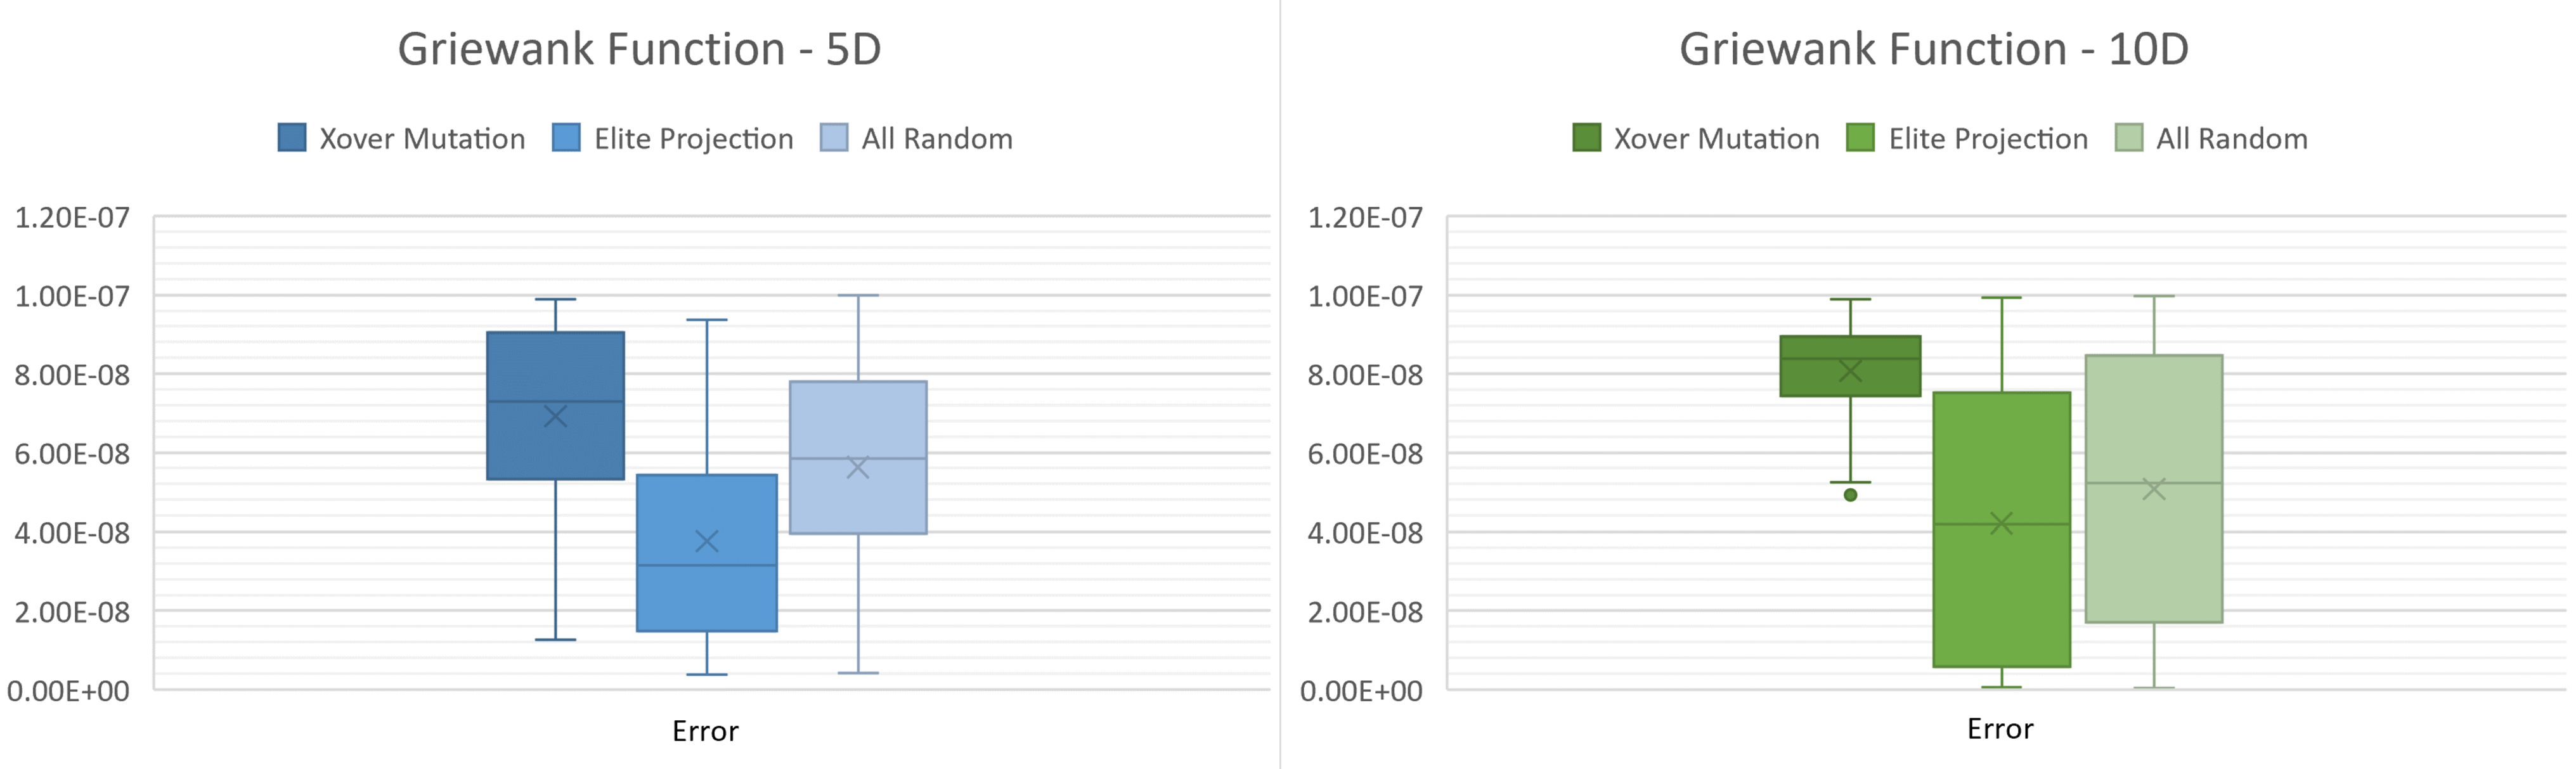
\includegraphics[width=0.99\linewidth, frame]{img/fig_fun_griewank.pdf}
                \caption{Box and whisker chart for the Griewank Benchmark Function, 5 vs 10 Dimensions.} \label{fig.fun_griewank}
                \end{figure}

            \begin{table}[]
                \scriptsize
                \centering
                \caption{Griewank Benchmark Function summarized experiments table for 5 Dimensions.}\label{tab.fun_griewank5}
                \begin{tabular}{@{}lllll@{}}
                \toprule
                \multicolumn{5}{l}{\textbf{Griewank Function - 5 Dimensions}} \\ \midrule
                & \textbf{Error} & \textbf{St-Dev} & \textbf{Evals.} & \textbf{Time} \\
                \textbf{Xover Mutation} & 6.92E-08 & 2.40E-08 & 44,566 & 48.3 \\
                \textbf{Elite Projection} & 3.77E-08 & 2.74E-08 & 16,412 & 20.1 \\
                \textbf{All Random} & 5.63E-08 & 2.99E-08 & 35,761 & 38.5 \\ \bottomrule
                \end{tabular}
                \end{table}

            \begin{table}[]
                \scriptsize
                \centering
                \caption{Griewank Benchmark Function summarized experiments table for 10 Dimensions.}\label{tab.fun_griewank10}
                \begin{tabular}{@{}lllll@{}}
                \toprule
                \multicolumn{5}{l}{\textbf{Griewank Function - 10 Dimensions}} \\ \midrule
                & \textbf{Error} & \textbf{St-Dev} & \textbf{Evals.} & \textbf{Time} \\
                \textbf{Xover Mutation} & 8.07E-08 & 1.39E-08 & 92,885 & 100.0 \\
                \textbf{Elite Projection} & 4.21E-08 & 3.40E-08 & 13,534 & 17.3 \\
                \textbf{All Random} & 5.08E-08 & 3.54E-08 & 40,544 & 52.5 \\ \bottomrule
                \end{tabular}
                \end{table}

            \FloatBarrier


        \subsubsection{Rastrigin Benchmark Function Experiment}

            This experiment's goal was to follow and study the behavior of our
            proposed strategy, to repeat the results in the same order as
            expected, in a reduced number of both time and evaluations. We
            selected Rastrigin Classic Benchmark Function for Optimization for
            this experiment. Figure~\ref{fig.fun_rastrigin} shows its
            corresponding Box and Whisker chart, where we summarized the
            results in Tables~\ref{tab.fun_rastrigin5} and~\ref{tab.fun_rastrigin10} 
            (for five and ten dimensions, respectively).

            \begin{figure}
                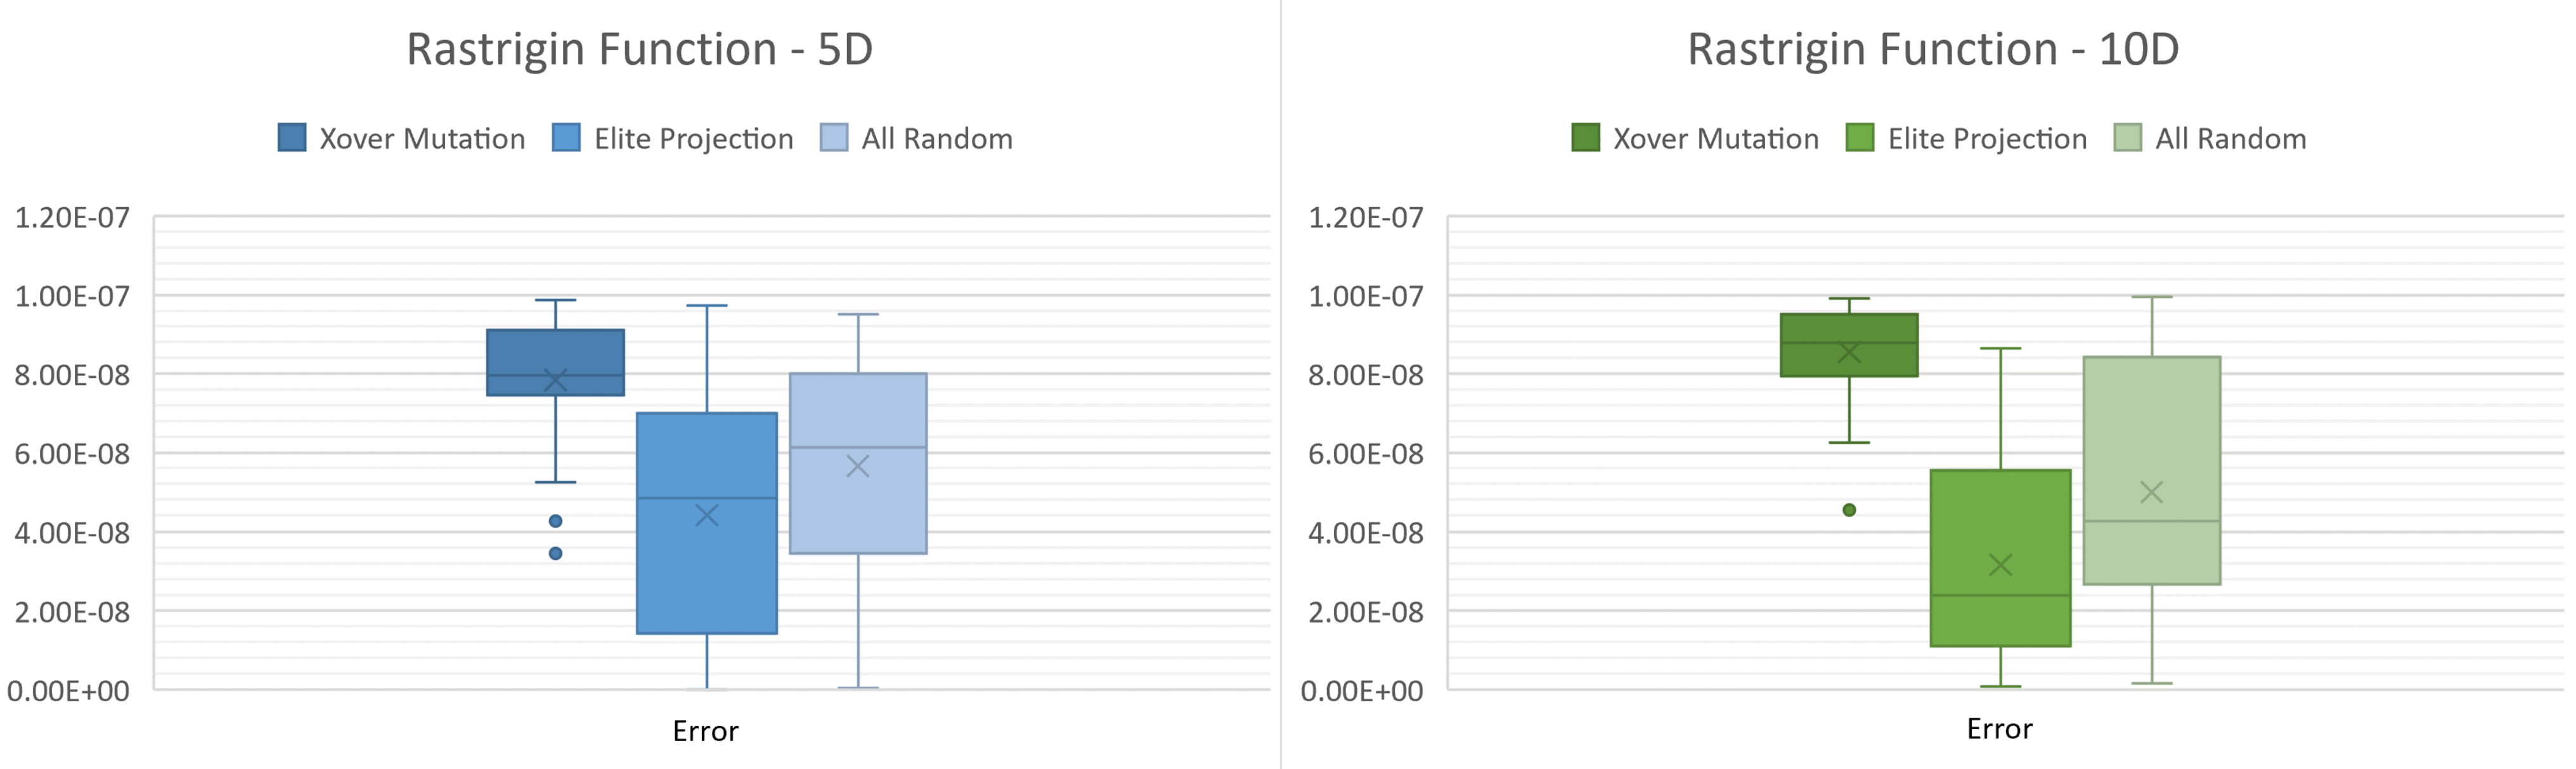
\includegraphics[width=0.99\linewidth, frame]{img/fig_fun_rastrigin.pdf}
                \caption{Box and whisker chart for the Rastrigin Benchmark Function, 5 vs 10 Dimensions.} \label{fig.fun_rastrigin}
                \end{figure}

            \begin{table}[]
                \scriptsize
                \centering
                \caption{Rastrigin Benchmark Function summarized experiments table for 5 Dimensions.}\label{tab.fun_rastrigin5}
                \begin{tabular}{@{}lllll@{}}
                \toprule
                \multicolumn{5}{l}{\textbf{Rastrigin Function - 5 Dimensions}} \\ \midrule
                & \textbf{Error} & \textbf{St-Dev} & \textbf{Evals.} & \textbf{Time} \\
                \textbf{Xover Mutation} & 7.85E-08 & 1.59E-08 & 22,322 & 34.1 \\
                \textbf{Elite Projection} & 4.42E-08 & 3.26E-08 & 10,860 & 14.8 \\
                \textbf{All Random} & 5.66E-08 & 2.81E-08 & 21,122 & 35.0 \\ \bottomrule
                \end{tabular}
                \end{table}

            \begin{table}[]
                \scriptsize
                \centering
                \caption{Rastrigin Benchmark Function summarized experiments table for 10 Dimensions.}\label{tab.fun_rastrigin10}
                \begin{tabular}{@{}lllll@{}}
                \toprule
                \multicolumn{5}{l}{\textbf{Rastrigin Function - 10   Dimensions}} \\ \midrule
                & \textbf{Error} & \textbf{St-Dev} & \textbf{Evals.} & \textbf{Time} \\
                \textbf{Xover Mutation} & 8.56E-08 & 1.23E-08 & 53,579 & 58.7 \\
                \textbf{Elite Projection} & 3.17E-08 & 2.57E-08 & 8,704 & 13.0 \\
                \textbf{All Random} & 5.00E-08 & 3.16E-08 & 24,376 & 27.4 \\ \bottomrule
                \end{tabular}
                \end{table}
            
            \FloatBarrier


        \subsubsection{Sphere Benchmark Function Experiment}

            For our fifth experiment we chose the Sphere Classic Benchmark
            Function for Optimization. Even though the sphere function is
            considered one of the simplest to solve, the same behavior was
            consistent for the algorithm, where it showed a reduced number of
            evaluations and execution time. We can confirm this affirmation
            with the results shown in this experiment.
            Figure~\ref{fig.fun_sphere} displays its corresponding Box and
            Whisker chart, where we summarized the results in
            Tables~\ref{tab.fun_sphere5} and~\ref{tab.fun_sphere10} (for
            five and ten dimensions, respectively).

            \begin{figure}
                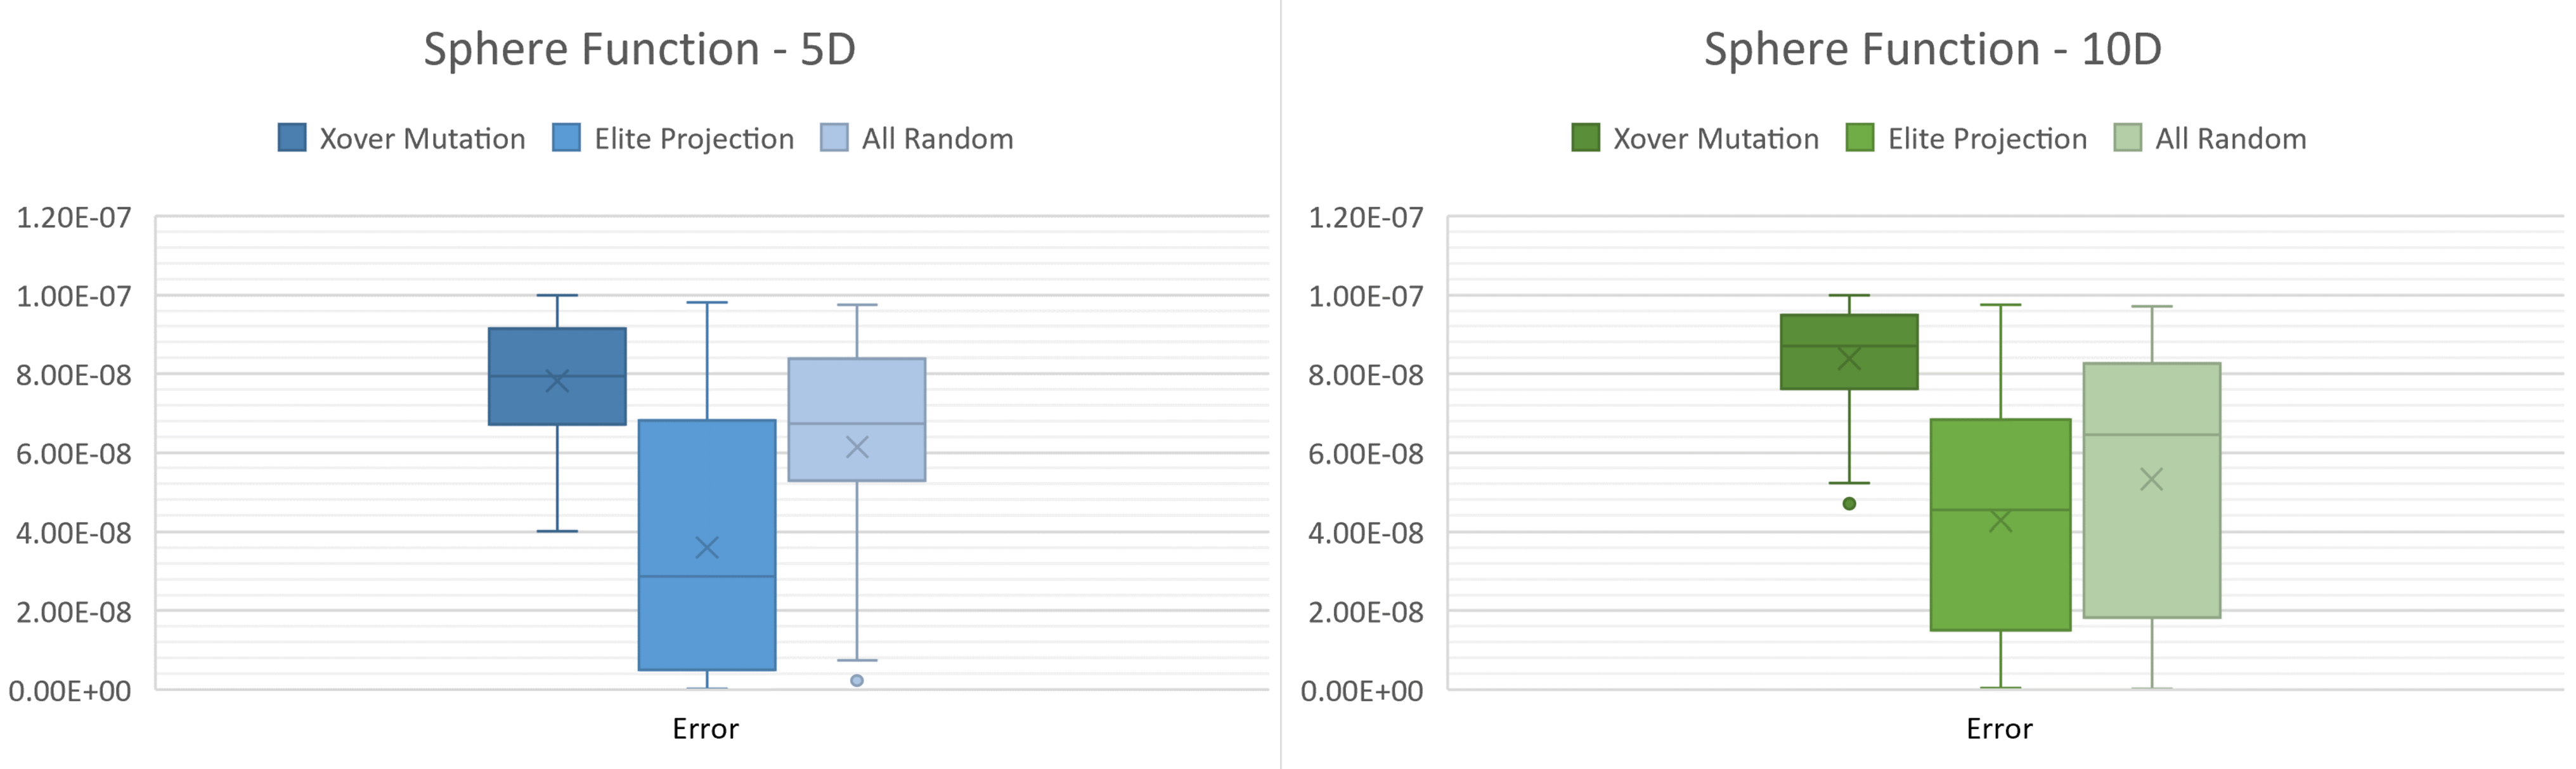
\includegraphics[width=0.99\linewidth, frame]{img/fig_fun_sphere.pdf}
                \caption{Box and whisker chart for the Sphere Benchmark Function, 5 vs 10 Dimensions.} \label{fig.fun_sphere}
                \end{figure}

            \begin{table}[]
                \scriptsize
                \centering
                \caption{Sphere Benchmark Function summarized experiments table for 5 Dimensions.}\label{tab.fun_sphere5}
                \begin{tabular}{@{}lllll@{}}
                \toprule
                \multicolumn{5}{l}{\textbf{Sphere Function - 5 Dimensions}} \\ \midrule
                & \textbf{Error} & \textbf{St-Dev} & \textbf{Evals.} & \textbf{Time} \\
                \textbf{Xover Mutation} & 7.82E-08 & 1.65E-08 & 11,312 & 14.5 \\
                \textbf{Elite Projection} & 3.60E-08 & 3.27E-08 & 7,056 & 10.9 \\
                \textbf{All Random} & 6.14E-08 & 2.79E-08 & 9,158 & 12.2 \\ \bottomrule
                \end{tabular}
                \end{table}

            \begin{table}[]
                \scriptsize
                \centering
                \caption{Sphere Benchmark Function summarized experiments table for 10 Dimensions.}\label{tab.fun_sphere10}
                \begin{tabular}{@{}lllll@{}}
                \toprule
                \multicolumn{5}{l}{\textbf{Sphere Function - 10 Dimensions}} \\ \midrule
                & \textbf{Error} & \textbf{St-Dev} & \textbf{Evals.} & \textbf{Time} \\
                \textbf{Xover Mutation} & 8.39E-08 & 1.45E-08 & 30,769 & 34.4 \\
                \textbf{Elite Projection} & 4.28E-08 & 3.06E-08 & 9,236 & 13.3 \\
                \textbf{All Random} & 5.32E-08 & 3.38E-08 & 21,465 & 26.3 \\ \bottomrule
                \end{tabular}
                \end{table}

            \FloatBarrier


        \subsubsection{Rosenbrock Benchmark Function Experiment}

            The goal of our sixth and last experiment was to study the behavior
            of the Animal Life-Cycle Algorithm when tested with the Rosenbrock
            Benchmark Function for Optimization. From all of our previous
            evaluation functions, Rosenbrock presented the most difficult
            challenge for our algorithm. This test facilitated the
            differentiation between the three compared strategies because the
            solutions found were in different numeric order. After all tests,
            the Elite Projection proved to be the best alternative. We can
            corroborate this by analyzing Figures~\ref{fig.fun_rosenbrock_5d}
            and~\ref{fig.fun_rosenbrock_10d}, which shows its corresponding Box
            and Whisker chart. We present the summarized results in
            Tables~\ref{tab.fun_rosenbrock5} and~\ref{tab.fun_rosenbrock10}
            (for five and ten dimensions, respectively).

            \begin{figure}
                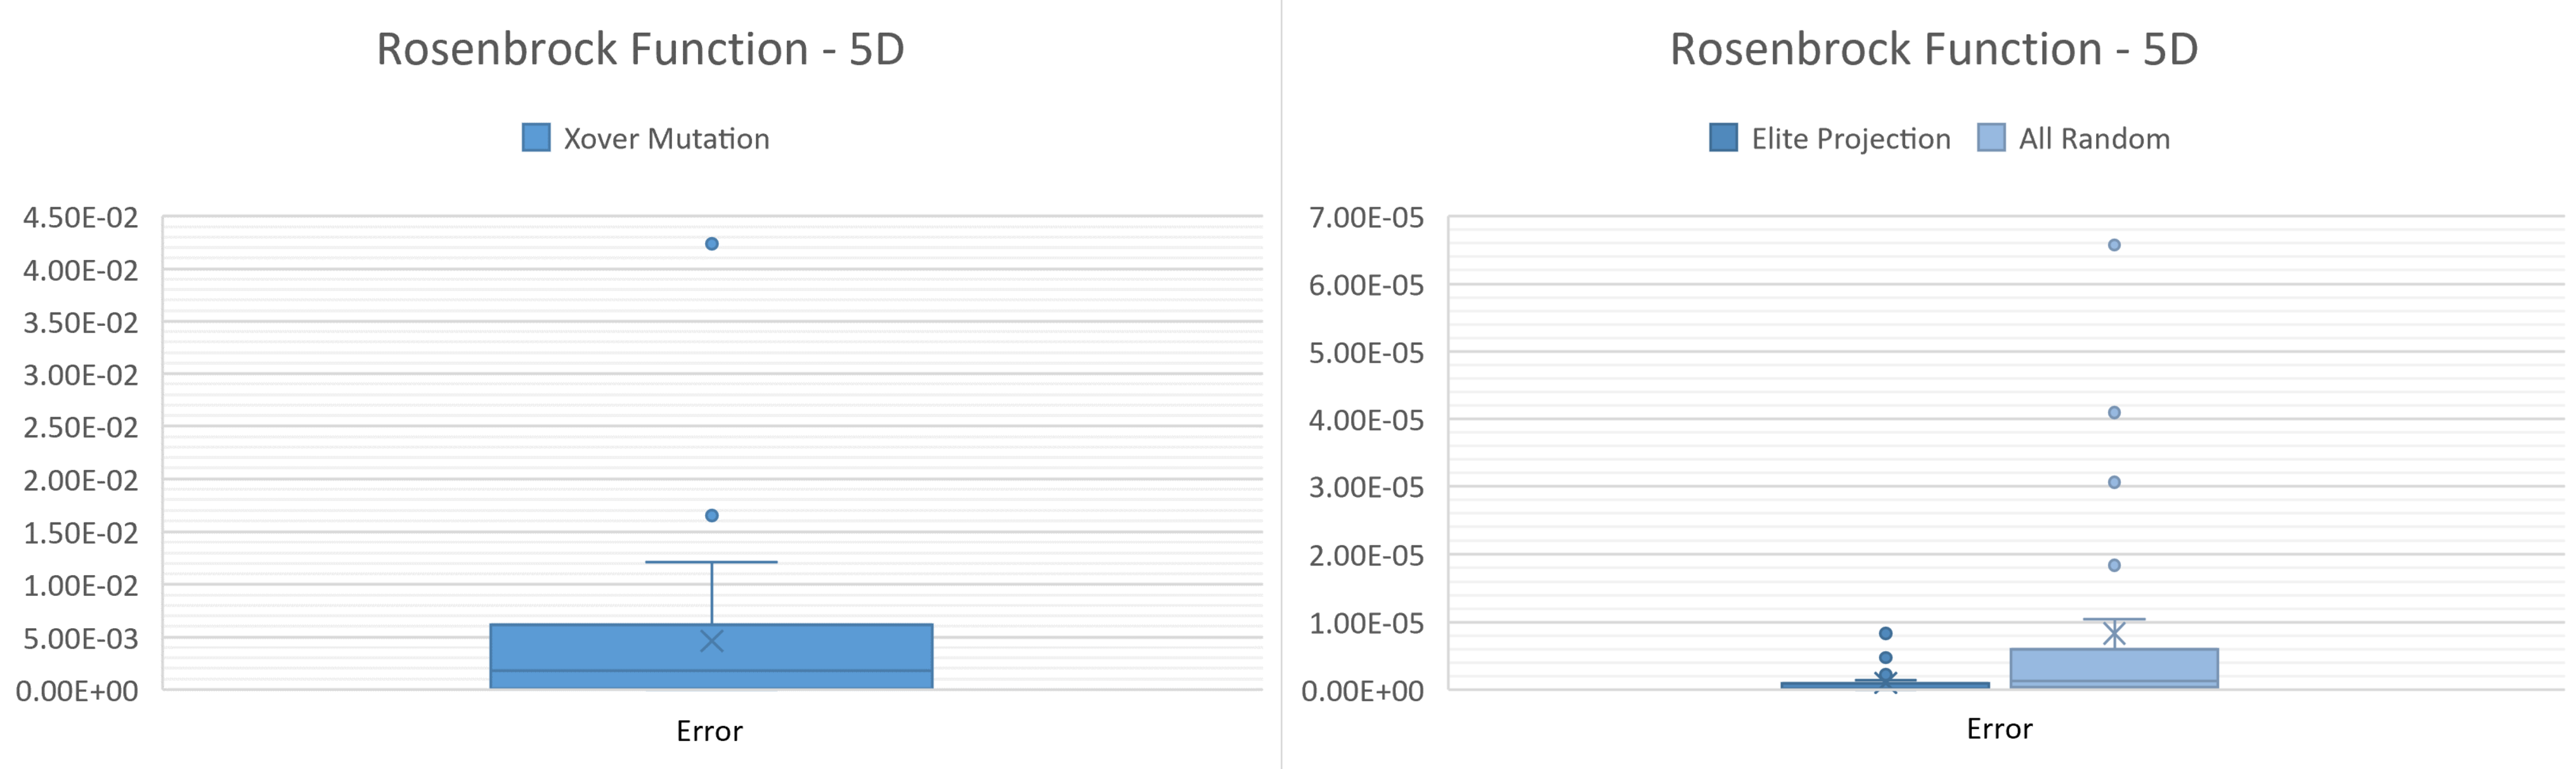
\includegraphics[width=0.99\linewidth, frame]{img/fig_fun_rosenbrock_5d.pdf}
                \caption{Box and whisker chart for the Rosenbrock Benchmark Function, 5 Dimensions.} \label{fig.fun_rosenbrock_5d}
                \end{figure}

            \begin{table}[]
                \scriptsize
                \centering
                \caption{Rosenbrock Benchmark Function summarized experiments table for 5 Dimensions.}\label{tab.fun_rosenbrock5}
                \begin{tabular}{@{}lllll@{}}
                \toprule
                \multicolumn{5}{l}{\textbf{Rosenbrock Function - 5 Dimensions}} \\ \midrule
                & \textbf{Error} & \textbf{St-Dev} & \textbf{Evals.} & \textbf{Time} \\
                \textbf{Xover Mutation} & 4.65E-03 & 8.29E-03 & 500,000 & 646.4 \\
                \textbf{Elite Projection} & 9.62E-07 & 1.86E-06 & 307,878 & 427.0 \\
                \textbf{All Random} & 8.30E-06 & 1.58E-05 & 491,400 & 697.8 \\ \bottomrule
                \end{tabular}
                \end{table}


            \begin{figure}
                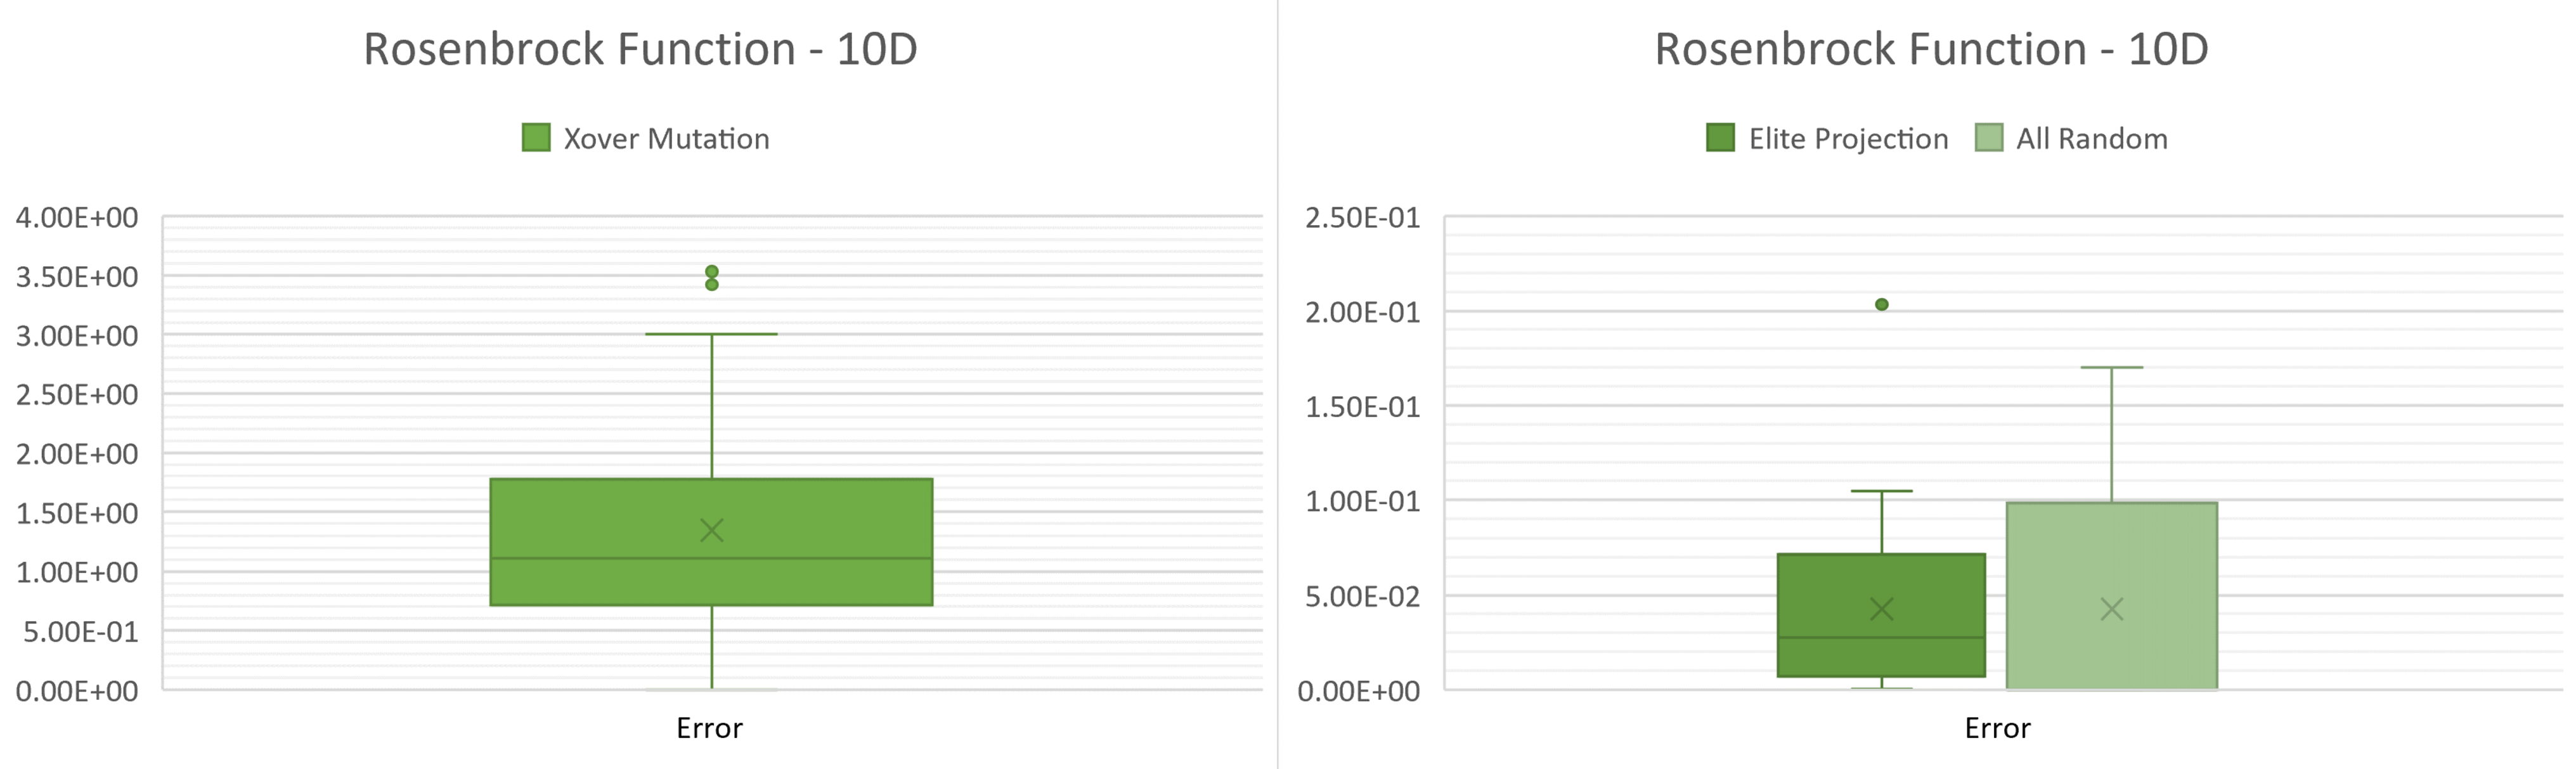
\includegraphics[width=0.99\linewidth, frame]{img/fig_fun_rosenbrock_10d.pdf}
                \caption{Box and whisker chart for the Rosenbrock Benchmark Function, 10 Dimensions.} \label{fig.fun_rosenbrock_10d}
                \end{figure}

            \begin{table}[]
                \scriptsize
                \centering
                \caption{Rosenbrock Benchmark Function summarized experiments table for 10 Dimensions.}\label{tab.fun_rosenbrock10}        
                \begin{tabular}{@{}lllll@{}}
                \toprule
                \multicolumn{5}{l}{\textbf{Rosenbrock Function - 10 Dimensions}} \\ \midrule
                & \textbf{Error} & \textbf{St-Dev} & \textbf{Evals.} & \textbf{Time} \\
                \textbf{Xover Mutation} & 1.35E+00 & 9.83E-01 & 1,000,000 & 1,384.3 \\
                \textbf{Elite Projection} & 4.26E-02 & 4.34E-02 & 1,000,000 & 1,146.0 \\
                \textbf{All Random} & 4.27E-02 & 6.02E-02 & 952,038 & 1,147.8 \\ \bottomrule
                \end{tabular}
                \end{table}
            
            \FloatBarrier

\section{Discussion}
    \label{section.discussion}

    Imagine being an astronaut on a mission repairing a space station in the
    middle of space. Suddenly, a block of asteroids hits the craft, and you
    lose your oxygen tank while the explosion pushes you away. From afar, you
    see the area where your tank might be, covered with something similar to a
    gas leaked from the station that blocks all visibility. Finding the tank is
    the only hope to return to your main ship some miles away. The oxygen
    reserve from your suit is running out, and there are only a couple of
    minutes left. Now hold your breath in real life and think, what strategy
    will you choose to search for your tank? We repeated this mental exercise
    several times until we found the best solution (or blacked out).

    If your life depended on it, would you choose a Genetic Algorithm, a
    variant of a Particle Swarm Optimization Algorithm, or another? We searched
    for a way to mix both, at least in some way, take the main idea or concepts
    from them and make them work together. We strongly believe it is possible
    to combine the features, as previous work has proven to obtain outstanding
    results \cite{garcia2015evospace,garcia2021event,valdez2021container,valdez2021swarm}.
    Our goal was to create a swarm out of the best individuals found in
    evolution. We probably have a long way to go, but at least we are getting
    promising results. From our experiments, all six Classic Benchmark
    Functions for Optimization (Ackley, Bohachevsky, Griewank, Rastrigin,
    Sphere, and Rosenbrock) proved the same behavior for the Animal Life Cycle
    Algorithm: finding the expected solution in a reduced number of evaluations
    and less execution time.


\section{Conclusions}
    \label{section.conclusions}

    The Animal Life Cycle Algorithm allows for multiple parameters'
    fine-tuning, facilitating the freedom to experiment with different
    alternatives to restart the population and solve extinction caused by
    nature's pressure, which will impact how quickly, and the quality of its
    found solution. We compared the results obtained with the use of historical
    elite projection versus other alternatives, using classic benchmark
    functions for optimization for comparison, where it showed favorable and
    promising results.

    As the nature of the challenge increases, it is indispensable to have an
    elastic, scalable, and fault-tolerant model designed with cloud
    collaboration processes, and asynchronous communication. We have proven
    that it is possible to evolve a population, using a distributed, parallel,
    and asynchronous strategy, inspired by the Genetic Algorithm (GA). To
    further validate this work, we could use some more demanding (or control)
    problem that requires calculating real numbers
    \cite{stanley2002evolving,miikkulainen2019evolving}. We implemented the
    algorithm using Docker containers.


\begin{acknowledgement}
    This paper has been supported in part by TecNM Project 15340.22-P.
\end{acknowledgement}

% ---- Bibliography ----
% BibTeX users should specify bibliography style 'splncs04'.
% References will then be sorted and formatted in the correct style.
%

\bibliographystyle{splncs03_unsrt}
%\bibliographystyle{splncs04}
\bibliography{bib/bibliografia.bib}

\end{document}

% TO-DO: Turnitin.
